\documentclass[a4paper]{scrartcl}
\usepackage[utf8]{inputenc}
\usepackage[english]{babel}
\usepackage{graphicx}
\usepackage{lastpage}
\usepackage{pgf}
\usepackage{wrapfig}
\usepackage{fancyvrb}
\usepackage{fancyhdr}
\pagestyle{fancy}

\usepackage[colorlinks=true,linkcolor=violet]{hyperref}
\usepackage[figure]{hypcap} %jump to img instead of caption text

\def\code#1{\texttt{#1}}

% Create header and footer
\headheight 27pt
\pagestyle{fancyplain}
\lhead{\footnotesize{Network Programming, ID1212}}
\chead{\footnotesize{Homework 5: Android Programming}}
\rhead{}
\lfoot{}
\cfoot{\thepage\ (\pageref{LastPage})}
\rfoot{}

% Create title page
\title{Homework 5: Distributed Applications Using Android}
\subtitle{Network Programming, ID1212}
\author{Max Körlinge, korlinge@kth.se}
\date{6 December 2018}

\begin{document}

\maketitle


\section{Introduction}

\noindent The assignment was to develop a distributed application where the client is an Android device. The focus was on designing, developing, and deploying an Android app using the Android SDK and IDE development tools. The game of Hangman was chosen as the implemented application. The requirements were:

\begin{itemize}
    \item The program must be designed using a layered architecture and object-oriented design principles.
    \item Some part of the application (for example, the client) must run on Android devices or emulators. There must be network communication from/to the nodes of the application running on Android.
    \item The Android app must have a responsive user interface, which means it must be multithreaded.
    \item The Android app must have a GUI developed using UI Views.
    \item Server must be multithreaded for the ability to handle several clients at once.
    \item The user interface must be informative, so the player knows what is going on.
\end{itemize}

The optional task was:

\begin{itemize}
    \item Use Firebase Cloud Messaging to communicate with the Android app. For example, to send a notification to the app. It was only required to handle the message on the Android client, and send the notification manually from the firebase cloud console.
\end{itemize}

The program was written in full by the author of this report and both the basic and optional tasks were completed.

\section{Literature Study}

To prepare for this assignment, all video material provided by the course on Android programming was viewed. After that, some time was spent reading the official Android documentation's guides to getting started with your first apps and on recommended Android app architecture, and also Firebase's guide to getting started with that. Important information was gathered on how to set up Android Studio and how to code in Android.

\section{Method}

\noindent Since there was no requirement to develop a new server, the server code from homework 1's implementation of Hangman was used as the game server for this application as well. The Android client was written in Android Studio and the program was tested on an Android emulator using Oreo 8.1 version of Android.

Development was done from the top down, that is, first, the \code{view} was made to work with a simple UI to get used to the IDE and Android way of things, then, the \code{viewmodel} was implemented, thirdly, the classes concerned with fetching data from the server and threading such calls were created, and lastly, the notification system with Firebase was implemented and a notification sent through the cloud console.

\section{Result}

\noindent The server source code can be found \href{https://github.com/fongie/Hangman/tree/master/hangmanserver}{here} whereas the Android client's source code, which this report is mostly concerned with, can be found at \href{https://github.com/fongie/AndroidHangman}{github.com/fongie/AndroidHangman}.

\begin{itemize}
    \item To comply with object-oriented design principles, the public interfaces are kept as small as possible, classes adhere to their specific purpose, and the number of dependencies for each class is kept at a minimum. Honestly, though, most methods implemented in the whole app are overridden methods and thus their definitions were decided before-hand by the Android API. 
        
        For architecture and layering, the Android \href{https://developer.android.com/jetpack/docs/guide}{guide to app architecture} was loosely followed. There is a \code{view} package containing Activities and Fragment, only dealing with the UI. After that, there is a \code{viewmodel} package, which holds the data currently displayed on the UI. This is accomplished using \code{LiveData} wrappers, which are basically implementations of the observer pattern, provided by Android. The UI observes these data wrappers and \href{https://github.com/fongie/AndroidHangman/blob/master/app/src/main/java/se/kth/korlinge/androidhangman/view/CurrentGameFragment.java#L80}{updates the UI when the data changes}. This way, the \code{view} does not have to contain any logic besides updating the UI.

        The \code{viewmodel} makes use of the \code{repository} layer to fetch its data. This layer, consisting of the \href{https://github.com/fongie/AndroidHangman/blob/master/app/src/main/java/se/kth/korlinge/androidhangman/repository/GameRepository.java}{GameRepository}, is responsible for fetching data. As such, since we fetch data via sockets and cannot block the UI, it also handles threading. To make the connection to the server, the repository calls on a class \code{Connection} in the \code{integration} package which does low-level socket management. The \code{integration} package also contains the service that handles Firebase integration. Lastly, there is a utility package \code{DTO} which contains data transfer objects, necessary for the communication between client and server to work.

    \item Some part of the application was required to run on Android and there had to be network communication. As you can see in the github repository, the client is an Android project, and as you can see in the \href{https://github.com/fongie/AndroidHangman/blob/master/app/src/main/java/se/kth/korlinge/androidhangman/integration/Connection.java}{Connection} class, there is network communication both from and to the Android client.

    \item The Android UI had to be responsive and use threading to accomplish this. All server communication is made in separate threads like \href{https://github.com/fongie/AndroidHangman/blob/master/app/src/main/java/se/kth/korlinge/androidhangman/repository/GameRepository.java#L38}{this} using the \code{CompletableFuture} class which means that the server communication runs in the common thread pool and does not block the UI. The observer pattern provided by the \code{LiveData} wrappers make sure that the \code{viewmodel} is updated when the thread finishes the server call.

    \item The Android app was required to have a GUI using UI Views. The main fragment and game UI is the \href{https://github.com/fongie/AndroidHangman/blob/master/app/src/main/java/se/kth/korlinge/androidhangman/view/CurrentGameFragment.java}{CurrentGameFragment}, and you can see pictures of the GUI in Figure 1.

    \item The server had to be able to handle multiple clients. Refer to Homework 1 to see a full explanation on the server, which is multithreaded, the threading happens \href{https://github.com/fongie/Hangman/blob/master/hangmanserver/src/main/java/net/Server.java#L53}{here}. As a bonus, this server can now simultaneously handle clients playing from both the Android app and the console client program developed in homework 1.
        
    \item The user interface had to be informative. See the left and middle pictures in Figure 1, which should show that the UI is informative enough.

    \item For the optional task, you had to send a message to the app using the Firebase console, and the app had to handle it. In Figure 1, on the far right, you can see the notification that was \href{https://github.com/fongie/AndroidHangman/blob/master/app/src/main/java/se/kth/korlinge/androidhangman/integration/MyFirebaseMessagingService.java#L31}{created by the app} after receiving a message sent manually from the Firebase console.

\end{itemize}

\begin{figure}[h!]
    \begin{center}
        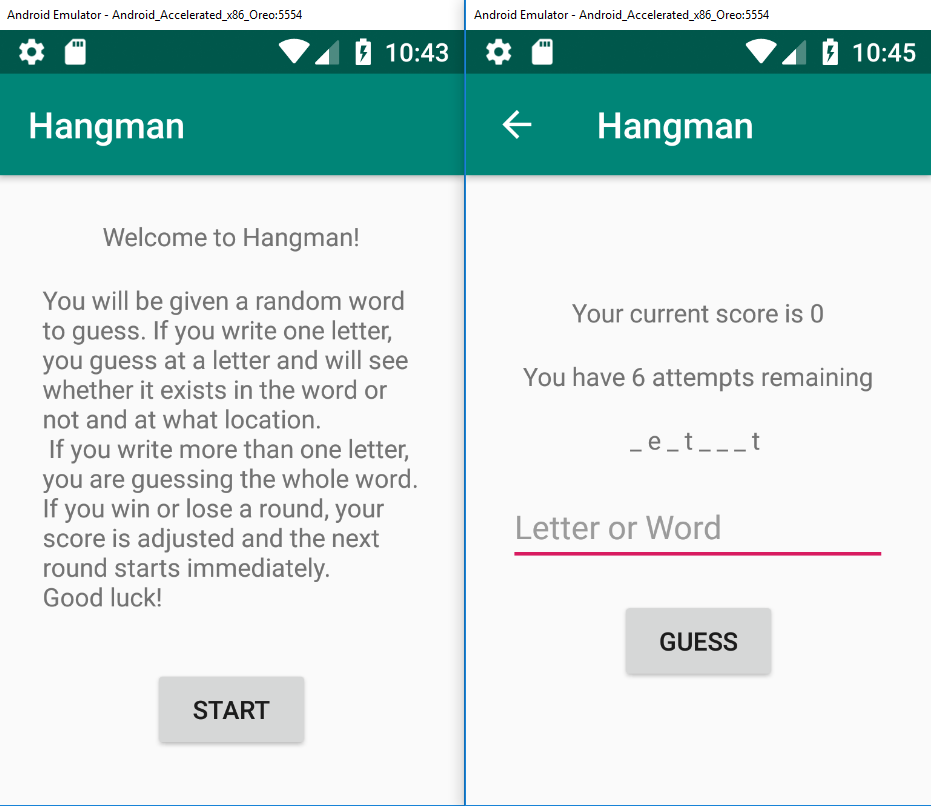
\includegraphics[scale=0.45]{ui.png}
        \caption{A sample output of the user interface}
        \label{fig:ui}
    \end{center}
\end{figure}

\section{Discussion}

This assignment was centered around learning about using the Android SDK in distributed applications. There were requirements on good architecture, developing a responsive GUI, and network communications on the Android device. There was an optional task to handle Firebase cloud messaging in the app. As presented above, all the basic requirements and the requirements of the optional tasks were met with.

My method in developing this Android application was rather less structured than previous assignments, because it was a bit of a pain to set up Android development with the Studio and emulator, and then try to wrap your head around all the classes that need to be extended and all the lifecycle methods in the view that have to be overridden and dealt with. That meant that the start of development consisted mostly of following some official get-started guides by Android, and then modifying the resulting classes to do what was required for this application instead. Since I have not developed an Android application before, this was a learning experience and took some time to get up and running with manifests, build files, string resources, etc. Once the GUI was finished with its viewmodel, and I found the guide to android app architecture, it went more smoothly to implement the underlying logic and server communication.

Given more time, I could improve the prettiness of the GUI, and use the server to programmatically send notifications through Firebase. An example would be to send a notification congratulating the user when winning a game and scoring a point. However, it was not required, so I decided to move on.

\section{Comments About the Course}

I spent about 2 hours on the lecture material, and about 12 hours on the assignment, including time spent with the official documentation, and 2 hours on the report, making 16 hours in total.

\end{document}
